\documentclass[conference]{IEEEtran}
\usepackage{times}

% numbers option provides compact numerical references in the text. 
\usepackage[numbers]{natbib}
\usepackage{multicol}
\usepackage[bookmarks=true]{hyperref}
\usepackage{color}
\usepackage{graphicx}

%% Tarik's Shortcuts
% For marking TODOs in an obvious way
\newcommand{\TODO}[1]{ {\bf \textcolor{red}{TODO:} #1 }}

\begin{document}

% paper title
\title{Computer-aided design of complex configurations and behaviors for modular robots}

% You will get a Paper-ID when submitting a pdf file to the conference system
\author{Author Names Omitted for Anonymous Review. Paper-ID [add your ID here]}

\maketitle

\begin{abstract}
In this paper, we present a scalable software framework for the design of modular robot configurations and behaviors. Designs are constructed hierarchically by composing elements from a library, allowing users to easily create complex designs.  Likewise, complex behaviors are constructed by composing controllers from a library in a nested series/parallel structure. The system is integrated with a full dynamic simulator, and provides tools to identify common problems with behaviors, specifically self-collision and loss of quasi-static stability.

\end{abstract}

\section{Introduction}
\TODO{ Tarik writes} \\

Modular reconfigurable robot systems have been studied extensively for several decades \TODO{citations}.  These systems distinguish themselves in their ability to transform into different shapes to address a wide variety of tasks. This flexibility places an additional burden on the user, who must design and program many configurations for different tasks.  In this paper, we introduce a software system to allow a user to easily build complex modular robot configurations by composing elemental units from a library, and program those designs by composing elemental controllers in a nested series/parallel fashion.  The system assists the user in verifying the correctness of designs and behaviors in a dynamic simulator by identifying self-collision and loss of quasi-static stability.

The primary contribution of this paper is a software framework that allows modular robot configurations and behaviors to be built hierarchically, and a simulation environment that helps the user verify intended behavior.  Together, these tools help manage the complexity of a modular robot system, significantly reducing the time and effort required to accomplish tasks.

We have developed our system for the SMORES modular robot, developed at the University of Pennsylvania \cite{Davey2012}. Each SMORES modules has four DoF (DoF) - three continuously rotating faces we call {\em turntables} and one central hinge with a $180^o$ range of motion (Figure~\ref{fig:SmoresRobot}). The DoF marked 1, 2, and 4 have rotational axes that are parallel and coincident. SMORES modules may connect to one another via magnets on each of their four faces, and are capable of  self-reconfiguration.

Note that while we demonstrate our software with SMORES, it is not limited to the SMORES robot - it could be applied to any modular robot which may be simulated using Gazebo.

\TODO{Related work here}


\begin{figure}[tb]
    \begin{center}
        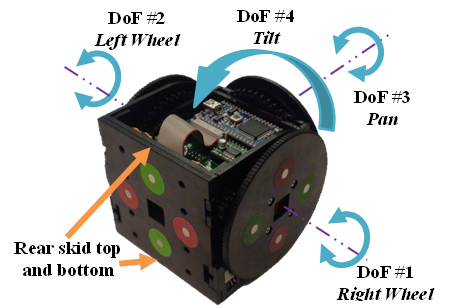
\includegraphics[width=\columnwidth]{images/smores_robot.png}
    \end{center}
    \caption{SMORES robot}
    \label{fig:SmoresRobot}
\end{figure}

\section{Preliminaries}
\TODO{Tarik writes}\\
Here we present preliminaries and define terms we will use later on in the paper.

A modular robot \textit{configuration} is a contigous set of connected modules.  A configuration is defined by its connective structure, represented by a topology graph. \TODO{Define the graph}.

A \textit{behavior} for a modular robot is a programmed sequence of movements intended to produce a desired effect (such as walking). In this work, we represent open-loop kinematic behaviors using a \textit{gait table} data structure, which contain a time series of joint-angles for a specific configuration \cite{yim1994locomotion}.  In this paper, we consider only behaviors that can be represented using gait tables. \TODO{This is the typical definition of gait tables.  Ours are actually more complicated.  We need to come up with a careful definition for them.}

A \textit{controller} is a position and velocity servo for one DoF of a modular robot.  A controller takes as input a desired position or angular velocity, and drives the error between the desired and actual state of the DoF it controls to zero over time.

When writing a behavior, it is possible to mistakenly command one controller to simultaneously hold more than one desired position; this is known as a \textit{controller conflict}.  Behaviors with controller conflicts are impossible to execute.

During execution of a behavior, a \textit{self-collision} can occur when two different parts of configuration are commanded to occupy the same location in space.  Self-collisions can damage the robot, and are usually unwanted.

In many cases, it is desirable to maintain \textit{quasi-static stability} during execution of a behavior \TODO{define}.

\section{Approach and Algorithm}
\TODO{Tarik and Jim write (see subsections)}
\paragraph{Configuration composition}
Define the composition of a set of configurations to a single configuration.

\subsection{Configuration Composition}
\TODO{Jim writes}
\paragraph{Input}
A set of configurations. A topology graph representing the connectivity among those configurations. A base module (for position transformation).
\paragraph{Output}
A composed configuration if it is safe.
\paragraph{Procedure}
\begin{itemize}
\item Start from the configurations that connects to the configuration with base module, transform their positions based on the position of the base configuration and topology graph.
\item Check if there is any collisions among the modules and report such collision.
\item \textbf{Check if the final configuration is stable. If not, find the plane that will make the configuration stable and transform the configuration.}
\item Show the expected behavior in simulator.
\end{itemize}

\paragraph{Controller composition}
Define the composition of a set of controllers to a single controller. Define the difference between a parallel composition and a series composition. Define the control composition graph.

\subsection{Controller Composition}
\TODO{Tarik and Jim write}
\paragraph{Input}
A configurations. A set of controllers. A control composition graph.
\paragraph{Output}
A composed controller if it is safe.
\paragraph{Procedure}
\begin{itemize}
\item Compose the set of controllers based on the given control composition graph. Explain how the parallel composition and series composition are handled.
\item\textbf{Check there is no controller conflict in the composition.}
\item Execute the composed controller in user defined incremental time interval. At each time step, update each module position and check collision.
\item \textbf{At each time step, check if the configuration will not have any unexpected behavior.}
\end{itemize}

\subsection{Complexity}
Discuss the complexity of the algorithm with respect to the number of modules and size of gait tables.

\section{Example and Experiment}
\TODO{Jim writes}\\
With simulation in Gazebo:
\begin{itemize}
\item Show a configuration composed from a set of basic configurations.
\item Show a composed controller that results in a collision in the configuration.
\item Show an updated controller that resolves the collision
\item Show a composed controller that results in an unexpected behavior.
\item Show an updated controller that eliminates the unexpected behavior.
\end{itemize}

\section{Conclusions}
We worked hard, and had fun.

\section{Future}
\begin{itemize}
\item How to represent different attribute/ability of the configurations
\end{itemize}




%% Use plainnat to work nicely with natbib. 

\bibliographystyle{plainnat}
\bibliography{references}

\end{document}


